\chapter{Méthodes}

\section{Développement et validation de la méthode ELISA de dosage du cetuximab.}

\subsection{Principes de l'ELISA indirect}

Nous avons développé et validé une méthode de mesure des concentrations sériques de cetuximab par ELISA indirecte (Publication~II). Les différentes étapes de cette méthode schématisées sur la Figure 17 sont les suivantes :
\begin{itemize}
\item la sensibilisation des puits de la plaque (une ligne sur deux) avec de l'EGFR recombinant.
\item la saturation de tous les puits avec de l'albumine pour limiter les fixations non spécifiques.
\item le dépôt des échantillons éventuellement dilués dans du sérum. 
\item le dépôt du conjugué qui est une portion F(ab)'2 d'anticorps de Chèvre couplée à une peroxydase et qui reconnait spécifiquement la chaîne ? des IgG humaines. 
\item le dépôt du substrat, un mélange de peroxyde d'hydrogène (H$_2$O$_2$) et d'ortho-phénylène diamine (OPD).
\item La réaction chimique catalysée par la peroxydase qui donne de l'eau (H$_2$O) et du 
2-3~diaminophénazine (coloration jaune).
\item Arrêt de la réaction par de l'acide sulfurique (H$_2$SO$_4$) qui dénature les protéines.
\item Lecture de l'absorbance à 492 et 620~nm puis interprétation.
\end{itemize}

\begin{landscape}
\begin{figure}[htbp]
	\centering
		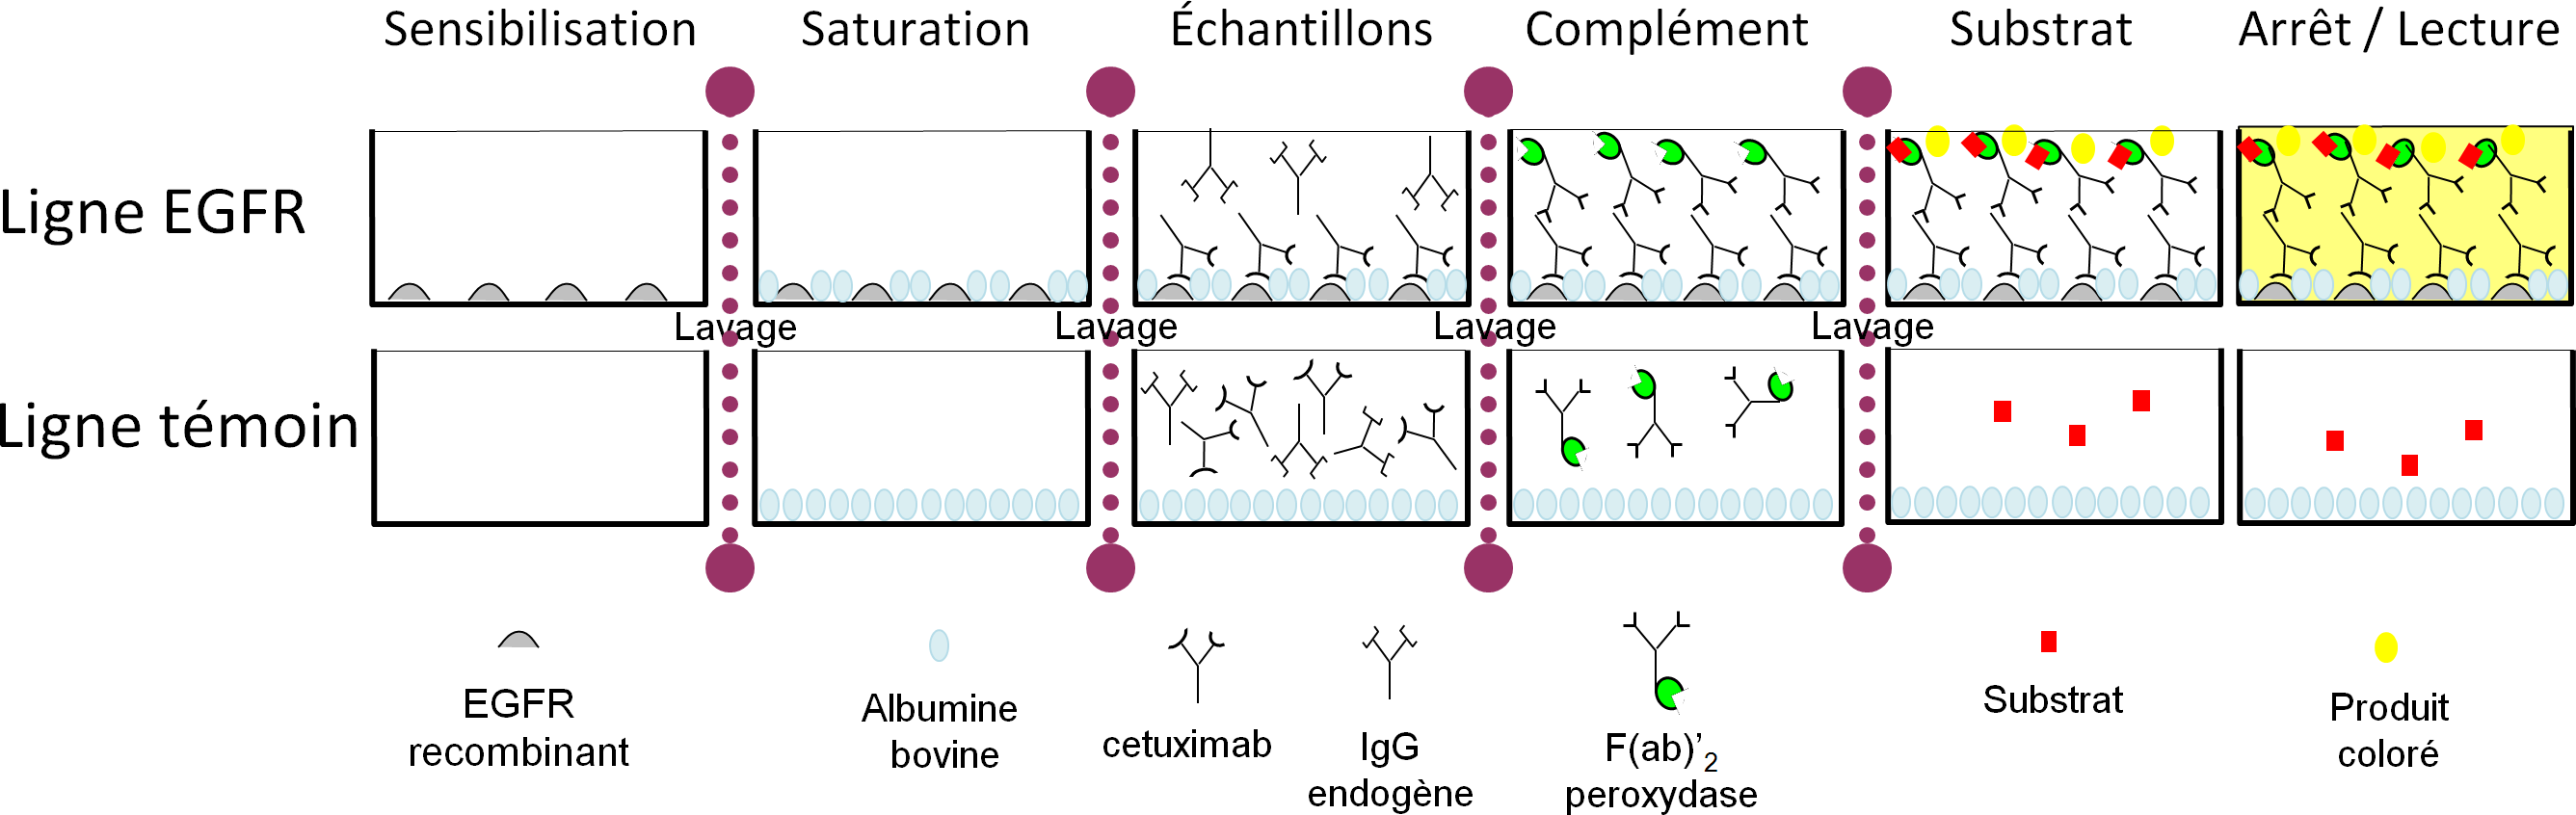
\includegraphics[width=20cm]{figures/raster/FIG_17}
	\caption[Étapes de la technique ELISA de dosage du cetuximab.]{Étapes de la technique ELISA de dosage du cetuximab. Chaque échantillon était déposé en double, dans un puits contenant de l'EGFR et dans un puits témoin sans EGFR. Pour chaque plaque, la mesure de 9 points de calibration et de 3 points de contrôle était réalisée. Avec une plaque de 96 puits, il était ainsi possible d'estimer la concentration de cetuximab de 12 échantillons de sérum.}
	\label{fig:17}
\end{figure}
\end{landscape}

\subsection{Développement}
Après avoir testé sans succès deux EGFR recombinants disponibles dans le commerce, nous avons produit notre propre EGFR recombinant. La mise au point et l'optimisation de cette production ont été réalisées par F. Piller (CNRS, Centre de Biophysique Moléculaire UPR~4301, Orléans, France). Des cellules HEK (cellules de rein de Hamster) ont été transfectées par un plasmide codant pour l'EGFR. Des modifications dans la séquence ont été apportées pour que la protéine soit sécrétée dans le surnageant et un \textit{tag} histidines a été ajouté pour permettre la purification sur billes de nickel. L'EGFR obtenu avait une concentration de l'ordre de 1~g/L.

A l'aide de sérums de 28 patients n'ayant jamais reçu de cetuximab, La limite de détection (LOD) était déterminée à 0,012~mg/L grâce à l'équation suivante :
\begin{equation}
54
\end{equation}
où  est la concentration moyenne estimée pour les sérums de patients n'ayant jamais reçu de cetuximab et  est l'écart-type. 

Les concentrations des points de calibration ont été réparties de façon régulière sur l'échelle logarithmique des concentrations entre 0 et 30~mg/L. La courbe de calibration était obtenue par régression logistique à l'aide de l'équation suivante :
\begin{equation}
55
\end{equation}
où $Abs$ était l'absorbance, et $A$, $B$, $C$, $N$ des constantes.
La réciproque de cette équation permettait de déduire les concentrations à partir des absorbances :
\begin{equation}
56
\end{equation}
La méthode de dosage du cetuximab par ELISA a été développée conformément aux recommandations publiées sur le développement des méthodes d'analyse des biomolécules par fixation à un ligand~\citep{REF133}. Ces recommandations préconisent une précision et un biais des concentrations estimées n'excédant pas 20\%.

De façon générale, le calcul de la précision est exprimé en pour-cent, par le coefficient de variation $P$ :
\begin{equation}
57
\end{equation}
où et sont respectivement la moyenne et l'écart-type empirique.

Le biais $B$ est quantifié par l'équation suivante :
\begin{equation}
58
\end{equation}
où $\mu$ est la valeur théorique.

Les concentrations des points de contrôle bas et haut étaient choisies pour donner une incertitude inférieure à 20\%. Ces points de contrôle déterminaient ainsi les limites de quantification basse (Lower limit of quantitation, LLOQ) et haute (Upper limit of quantitation, ULOQ). En deçà de la LLOQ, la concentration était censurée, c'est-à-dire exprimée comme inférieure à la LLOQ. Les incertitudes et les biais des contrôles de qualité bas (0,75~mg/L) et haut (15~mg/L) étant inférieurs à 15\%, ces concentrations ont été définies respectivement comme étant les limites de quantification LLOQ et ULOQ.
\subsection{Validation de la méthode}
La répétabilité intra-jour et inter-jour de la méthode a été contrôlée. La précision et le biais de chaque contrôle de qualité étaient analysés au moins 5 fois le même jour (intra-jour) et une fois pendant au moins 5~jours consécutifs (inter-–jour). L'étude de la reproductibilité intra-jour et inter-jour a montré que la précision et le biais de toutes les concentrations de calibration et de contrôle (en dehors de 0 et 0,1~mg/L) étaient inférieures à 20\% (Article 1, Tableau 1).
\subsubsection{Contrôle de dilution}
Parfois, une concentration sérique d'anticorps pouvait être supérieure à ULOQ (en particulier juste après une perfusion). L'échantillon à mesurer était alors dilué dans du sérum au 10éme ou au 100ème. Puisque cette dilution était une source de variabilité, la reproductibilité des dilutions au 10ème et au 100ème a été testée pour différents sérums surchargés en cetuximab. La précision de la dilution était contrôlée avec des échantillons de sérum surchargés en cetuximab afin d'obtenir les concentrations de 50, 200 et 300~mg/L. Les moyennes, CV et imprécisions des concentrations estimées sont reportés dans le tableau ci-dessous :

\begin{table}[!ht]
  \centering
  \caption{Contrôle de de la reproductibilité des dilutions avec respectivement $\mu$ et $\bar{\mu}$ les concentrations théoriques et moyennes estimées.}
    \begin{tabular}{lcclcc}
    &&&&&\\
      \hline
      \textbf{$\mu$} & \textbf{dilution} & \textbf{échantillons} & \textbf{$\bar{\mu}$} & \textbf{CV} & \textbf{imprécision} \\
      \hline
      \hline
      50 & 1/10 & 5 & 51,5 & 4,5 \% & +3,1\% \\
      200 & 1/100 & 5 & 205,3 & 2,6 \% & +2,6\% \\
      300 & 1/100 & 5 & 291,9 & 5,5 \% & +2,7\% \\
      \hline
    \end{tabular}
  \label{tab:3}
\end{table}

\subsubsection{Spécificité}
La spécificité de la méthode de dosage pour le cetuximab a été contrôlée avec des sérums contenant des facteurs rhumatoïdes, des IgG et d'autres anticorps thérapeutiques (infliximab, bevacizumab, rituximab). Parmi les cinq serums contenant des facteurs rhumatoïdes issus de patients n'ayant jamais été traités par cetuximab, aucun n'a montré une absorbance correspondant à une concentration supérieure à la LOD. Parmi les cinq serums contenant une concentration élevée d'IgG issus de patients n'ayant jamais été traités par cetuximab, un seul a montré une absorbance correspondant à une concentration supérieure à la LOD (0,012~mg/L), mais elle était inférieure à la LLOQ (0,75~mg/L). Les sérums de sujets sains surchargés avec de l'infliximab, du bevacizumab ou du rituximab, n'ont pas montré d'absorbance correspondant à une concentration supérieure à la LOD.
\section{Modélisation de la pharmacocinétique}
\subsection{Choix de l'approche de modélisation}
Dans les études de cette thèse, les trois approches non-compartimentale, compartimentale individuelle et compartimentale de population ont été utilisées. L'approche non-compartimentale était utilisée pour disposer de valeurs initiales pour les paramètres du modèle compartimental. L'approche compartimentale individuelle était utilisée lorsque les données étaient "riches" et permettaient une description correcte des concentrations. Les données de l'étude de la pharmacocinétique du cetuximab dans le cancer colorectal métastatique (publications~II et III) étaient trop "pauvres" pour une approche non-compartimentale ou compartimentale individuelle. Cependant, le nombre de patients était suffisamment important pour permettre une analyse compartimentale de population et ainsi rechercher les covariables influençant la pharmacocinétique du cetuximab. 
\subsection{Choix du modèle structural et de variabilité interindividuelle}
Dans chaque étude, des modèles à un et deux compartiments, avec constantes de transfert d'ordre~1 et constante(s) d'élimination d'ordre~0 et/ou d'ordre~1 ont été testés. Dans l'étude de la pharmacocinétique de la publication~III, un modèle à deux compartiments avec élimination mixte d'ordre~1 et de type Michaelis-Menten a également été testé. Le modèle structural retenu était celui qui présentait les meilleures performances descriptives et permettait une diminution significative de la fonction objective.

La variabilité interindividuelle des paramètres structuraux était décrite par un modèle exponentiel (équation~\ref{eq:46}).

L'évaluation du modèle final était basée sur l'inspection graphique (\textit{goodness of fit plot})  et sur l'analyse des erreurs standards des paramètres obtenus (r.s.e.\%).
\subsection{Choix du modèle d'erreur résiduelle}
Le choix du modèle d'erreur résiduelle était déterminé par la diminution significative de la $-2LL$ et par l'ajustement des concentrations prédites avec les concentrations observées. Dans les travaux de la publication~III, les modèles additif, proportionnel, mixte et exponentiel ont été testés.
\subsection{Sélection des covariables significatives}
Dans la publication~III, les covariables d'intérêt ont été analysées par une procédure pas à pas ascendante puis pas à pas descendante :
\begin{description}
\item[Pas à pas ascendante (ou Forward stepwise) :] En partant du modèle structural sans covariable, les covariables d'intérêt étaient testées l'une après l'autre. Si la diminution de la FO était significative ($p < 0,1$), la covariable était retenue dans le modèle. La covariable d'intérêt suivante était testée sur le modèle retenu.
\item[Pas à pas descendante (ou Backward stepwise) :] A la fin de l'étape Forward, après inclusion de toutes les covariables d'intérêt significatives, ces covariables étaient retirées une à une. Si le retrait d'une covariable ne faisait pas augmenter significativement la FO ($p < 0,05$), la covariable n'était pas retenue.
\end{description}
Les covariables continues étaient centrées sur leurs valeurs médianes. 
\section{Analyse de survie sans progression}
Le temps de survie sans progression (PFS pour \textit{progression-free survival}) est le temps de traitement pendant lequel le patient n'a pas progressé ou n'est pas décédé. Ce temps peut éventuellement être censuré, si le patient n'a pas encore progressé au moment de l'arrêt du suivi ou de l'analyse. On parle alors de censure "à gauche". La représentation graphique des temps de survie sans progression d'une cohorte de patients se fait par une courbe de Kaplan-Meier. Ce graphique représente le nombre relatif de patients n'ayant pas progressé en fonction du temps de traitement. L'expression la plus courante pour quantifier les PFS d'une cohorte de patients est le temps médian de survie sans progression qui correspond au temps après lequel la moitié des patients a progressé. Bien que cet indice soit fréquemment utilisé, il ne permet pas de caractériser globalement la fonction de survie.

La fonction de survie est la probabilité que la progression intervienne après un temps t donné. Elle est notée $S$ par convention et est définie par :
\begin{equation}
59
\end{equation}
où $t$ est le temps, $T$ est le temps de progression et $P$ est la fonction de probabilité.

La modélisation de la fonction de survie permet une description globale de la PFS mais également d'identifier des facteurs de variabilité. Cette modélisation peut se faire par approche paramétrique ou semi-paramétrique :
\begin{description}
\item[Approche paramétrique :] La distribution des temps de survie sans progression peut être décrite par une distribution de Weibull. La fonction de survie correspond alors à l'équation suivante : 
\begin{equation}
60
\end{equation}
où ? est le risque instantané de progression et $k$ le paramètre d'échelle. La recherche de covariables peut se faire comme pour l'analyse pharmacocinétique, sur les deux paramètres. 

Si le risque de progression augmente avec le temps, $k < 1$. Si ce risque diminue, $k > 1$. Lorsque $k = 1$, le risque de progression est constant au cours du temps ; la distribution des temps de survie est alors de type exponentiel.
\item[Approche semi-paramétrique :] Le modèle de Cox exprime la fonction de risque instantané de progression ?(t) en deux parties : 
\begin{equation}
61
\end{equation}
où ? est le risque de base qui dépend du temps mais pas des covariables et où  correspond à l'influence des n covariables sur le risque instantané. Ce modèle est dit semi-paramétrique, car on ne cherche pas à décrire, qui est par hypothèse le même pour tous les patients, mais plutôt les risques relatifs estimés par  pour la covariable~$i$.
\end{description}
Dans l'étude des données de survie sans progression de la publication~III, des approches paramétriques (distributions exponentielles et de Weibull) ont été testées pour décrire la distribution des temps de survie sans progression. L'approche semi-paramétrique par régression de Cox a permis d'évaluer les risques relatifs instantanés de progression. Toutes les variables continues testées étaient également dichotomisées par rapport à leurs médianes respectives, pour une interprétation et une illustration plus explicites des risques relatifs. 
\section{Simulations}
Pour étudier l'impact de l'espacement des injections de cetuximab sur sa pharmacocinétique, trois profils pharmacocinétiques obtenus avec différentes posologies ont été simulées. La surface corporelle de 1000~patients a été générée à l'aide d'une loi normale de moyenne égale à la surface corporelle médiane des patients de la publication~III (1,79 m$^2$) et une variabilité de 30\%. Ces surfaces corporelles étaient censurées à gauche et à droite en fonction des valeurs extrêmes de la publication~III (1,21 -- 2,27 m$^2$). A partir du modèle compartimental de population, également issus de la publication~III, les paramètres pharmacocinétiques de ces patients ont été générés. Pour être comparables, les simulations d'injection de 250, 500 et 750 mg/m$^2$ respectivement, toutes les une, deux ou trois semaines devaient se faire sur 84 jours (2 fois 3 semaines). Pour chaque heure, les concentrations étaient estimées dans les deux compartiments et l'$AUC$ dans le compartiment central.
\section{Outils informatiques}
Toutes les analyses statistiques étaient réalisées grâce au logiciel R~\citep{REF134}.

La modélisation non-compartimentale de la publication~V a été réalisée avec Excel 2007 et WinNonLin Professional~5.2 (Pharsight, Mountain View, USA). Les résultats obtenus ont facilité la modélisation compartimentale de population des données avec le logiciel WinNonMix Professional~2.0.1 (Pharsight, Mountain View, USA). La modélisation compartimentale individuelle de la publication~II a été réalisée avec WinNonLin. La modélisation compartimentale de population de la publication~III a été réalisée avec WinNonMix, NONMEM~6 et 7, puis publiée avec les résultats obtenus avec Monolix~3.2. 

Les analyses de survie ont été réalisées avec le logiciel R~\citep{REF134} et les « packages » \verb_survival_~\citep{REF134surv} et \verb_eha_~\citep{REF134eha}.
